% Options for packages loaded elsewhere
\PassOptionsToPackage{unicode}{hyperref}
\PassOptionsToPackage{hyphens}{url}
%
\documentclass[
]{book}
\usepackage{lmodern}
\usepackage{amssymb,amsmath}
\usepackage{ifxetex,ifluatex}
\ifnum 0\ifxetex 1\fi\ifluatex 1\fi=0 % if pdftex
  \usepackage[T1]{fontenc}
  \usepackage[utf8]{inputenc}
  \usepackage{textcomp} % provide euro and other symbols
\else % if luatex or xetex
  \usepackage{unicode-math}
  \defaultfontfeatures{Scale=MatchLowercase}
  \defaultfontfeatures[\rmfamily]{Ligatures=TeX,Scale=1}
\fi
% Use upquote if available, for straight quotes in verbatim environments
\IfFileExists{upquote.sty}{\usepackage{upquote}}{}
\IfFileExists{microtype.sty}{% use microtype if available
  \usepackage[]{microtype}
  \UseMicrotypeSet[protrusion]{basicmath} % disable protrusion for tt fonts
}{}
\makeatletter
\@ifundefined{KOMAClassName}{% if non-KOMA class
  \IfFileExists{parskip.sty}{%
    \usepackage{parskip}
  }{% else
    \setlength{\parindent}{0pt}
    \setlength{\parskip}{6pt plus 2pt minus 1pt}}
}{% if KOMA class
  \KOMAoptions{parskip=half}}
\makeatother
\usepackage{xcolor}
\IfFileExists{xurl.sty}{\usepackage{xurl}}{} % add URL line breaks if available
\IfFileExists{bookmark.sty}{\usepackage{bookmark}}{\usepackage{hyperref}}
\hypersetup{
  pdftitle={My Notes on Ula\&Smith (2009) Paper},
  pdfauthor={Peyman Kor},
  hidelinks,
  pdfcreator={LaTeX via pandoc}}
\urlstyle{same} % disable monospaced font for URLs
\usepackage{color}
\usepackage{fancyvrb}
\newcommand{\VerbBar}{|}
\newcommand{\VERB}{\Verb[commandchars=\\\{\}]}
\DefineVerbatimEnvironment{Highlighting}{Verbatim}{commandchars=\\\{\}}
% Add ',fontsize=\small' for more characters per line
\usepackage{framed}
\definecolor{shadecolor}{RGB}{248,248,248}
\newenvironment{Shaded}{\begin{snugshade}}{\end{snugshade}}
\newcommand{\AlertTok}[1]{\textcolor[rgb]{0.94,0.16,0.16}{#1}}
\newcommand{\AnnotationTok}[1]{\textcolor[rgb]{0.56,0.35,0.01}{\textbf{\textit{#1}}}}
\newcommand{\AttributeTok}[1]{\textcolor[rgb]{0.77,0.63,0.00}{#1}}
\newcommand{\BaseNTok}[1]{\textcolor[rgb]{0.00,0.00,0.81}{#1}}
\newcommand{\BuiltInTok}[1]{#1}
\newcommand{\CharTok}[1]{\textcolor[rgb]{0.31,0.60,0.02}{#1}}
\newcommand{\CommentTok}[1]{\textcolor[rgb]{0.56,0.35,0.01}{\textit{#1}}}
\newcommand{\CommentVarTok}[1]{\textcolor[rgb]{0.56,0.35,0.01}{\textbf{\textit{#1}}}}
\newcommand{\ConstantTok}[1]{\textcolor[rgb]{0.00,0.00,0.00}{#1}}
\newcommand{\ControlFlowTok}[1]{\textcolor[rgb]{0.13,0.29,0.53}{\textbf{#1}}}
\newcommand{\DataTypeTok}[1]{\textcolor[rgb]{0.13,0.29,0.53}{#1}}
\newcommand{\DecValTok}[1]{\textcolor[rgb]{0.00,0.00,0.81}{#1}}
\newcommand{\DocumentationTok}[1]{\textcolor[rgb]{0.56,0.35,0.01}{\textbf{\textit{#1}}}}
\newcommand{\ErrorTok}[1]{\textcolor[rgb]{0.64,0.00,0.00}{\textbf{#1}}}
\newcommand{\ExtensionTok}[1]{#1}
\newcommand{\FloatTok}[1]{\textcolor[rgb]{0.00,0.00,0.81}{#1}}
\newcommand{\FunctionTok}[1]{\textcolor[rgb]{0.00,0.00,0.00}{#1}}
\newcommand{\ImportTok}[1]{#1}
\newcommand{\InformationTok}[1]{\textcolor[rgb]{0.56,0.35,0.01}{\textbf{\textit{#1}}}}
\newcommand{\KeywordTok}[1]{\textcolor[rgb]{0.13,0.29,0.53}{\textbf{#1}}}
\newcommand{\NormalTok}[1]{#1}
\newcommand{\OperatorTok}[1]{\textcolor[rgb]{0.81,0.36,0.00}{\textbf{#1}}}
\newcommand{\OtherTok}[1]{\textcolor[rgb]{0.56,0.35,0.01}{#1}}
\newcommand{\PreprocessorTok}[1]{\textcolor[rgb]{0.56,0.35,0.01}{\textit{#1}}}
\newcommand{\RegionMarkerTok}[1]{#1}
\newcommand{\SpecialCharTok}[1]{\textcolor[rgb]{0.00,0.00,0.00}{#1}}
\newcommand{\SpecialStringTok}[1]{\textcolor[rgb]{0.31,0.60,0.02}{#1}}
\newcommand{\StringTok}[1]{\textcolor[rgb]{0.31,0.60,0.02}{#1}}
\newcommand{\VariableTok}[1]{\textcolor[rgb]{0.00,0.00,0.00}{#1}}
\newcommand{\VerbatimStringTok}[1]{\textcolor[rgb]{0.31,0.60,0.02}{#1}}
\newcommand{\WarningTok}[1]{\textcolor[rgb]{0.56,0.35,0.01}{\textbf{\textit{#1}}}}
\usepackage{longtable,booktabs}
% Correct order of tables after \paragraph or \subparagraph
\usepackage{etoolbox}
\makeatletter
\patchcmd\longtable{\par}{\if@noskipsec\mbox{}\fi\par}{}{}
\makeatother
% Allow footnotes in longtable head/foot
\IfFileExists{footnotehyper.sty}{\usepackage{footnotehyper}}{\usepackage{footnote}}
\makesavenoteenv{longtable}
\usepackage{graphicx}
\makeatletter
\def\maxwidth{\ifdim\Gin@nat@width>\linewidth\linewidth\else\Gin@nat@width\fi}
\def\maxheight{\ifdim\Gin@nat@height>\textheight\textheight\else\Gin@nat@height\fi}
\makeatother
% Scale images if necessary, so that they will not overflow the page
% margins by default, and it is still possible to overwrite the defaults
% using explicit options in \includegraphics[width, height, ...]{}
\setkeys{Gin}{width=\maxwidth,height=\maxheight,keepaspectratio}
% Set default figure placement to htbp
\makeatletter
\def\fps@figure{htbp}
\makeatother
\setlength{\emergencystretch}{3em} % prevent overfull lines
\providecommand{\tightlist}{%
  \setlength{\itemsep}{0pt}\setlength{\parskip}{0pt}}
\setcounter{secnumdepth}{5}
\usepackage{booktabs}
\ifluatex
  \usepackage{selnolig}  % disable illegal ligatures
\fi
\usepackage[]{natbib}
\bibliographystyle{apalike}

\title{My Notes on Ula\&Smith (2009) Paper}
\author{Peyman Kor}
\date{2020-11-13}

\begin{document}
\maketitle

{
\setcounter{tocdepth}{1}
\tableofcontents
}
\hypertarget{abstract}{%
\chapter{Abstract}\label{abstract}}

Consumers or firms contemplating purchasing a new product or adopting a new technology are often plagued by uncertainty: Will the benefits outweigh the costs? Should we buy now or wait and gather more information? In this paper, we study a dynamic programming model of this technology adoption problem. In each period, the consumer decides whether to adopt the technology, reject it, or wait and gather additional information by observing a signal about the technology's benefit. The technology's actual benefit may be constant or changing stochastically over time. The dynamic programming state variable is a probability distribution that describes the consumer's beliefs about the benefits of the technology. We allow general probability distributions on benefits and general signal processes and assume that the consumer updates her beliefs over time using Bayes' rule. We are interested in structural properties of this model. We show that improving the technology's benefit need not make the consumer better off and that first-order stochastic dominance improvements in the consumer's distribution on benefits need not increase the consumer's value function. Nevertheless, the model possesses a great deal of structure. For example, we obtain monotonic value functions and policies if we order distributions using
likelihood-ratio dominance rather than first-order stochastic dominance. We also examine convexity properties and provide many comparative statics results.

\hypertarget{model-implementation---part2.1}{%
\chapter{Model Implementation ( - Part2.1 )}\label{model-implementation---part2.1}}

\hypertarget{importing-the-required-library}{%
\section{Importing the required library}\label{importing-the-required-library}}

\begin{Shaded}
\begin{Highlighting}[]
\KeywordTok{library}\NormalTok{(tidyverse)}
\end{Highlighting}
\end{Shaded}

\hypertarget{model-parameters-definition}{%
\section{Model parameters definition}\label{model-parameters-definition}}

\(\theta:\)

the Net Present Value of Stream of benefits

\begin{itemize}
\item
  If she decides to reject the technology, she receives nothing and no longer gathers information about the technology.
\item
  If she decides to \emph{adopt} the technology, she pays a fixed adoption cost K and receives a net expected benefit:
\end{itemize}

\[\int_{\theta} \theta \pi(\theta)d\theta - K\]

\(\theta\) has the density \(\pi\).

\begin{itemize}
\tightlist
\item
  Now, if consumer choose to gather additional information, she pays \emph{c} \emph{in that period} and observe the signal x, drawn with likelihood function
\end{itemize}

\[L(x|\theta)\]

Having observed signal x, the consumer then updates her prior \(\pi\) using Baye's rule:

\[\prod(\theta;\pi,x) = \frac{L(x|\theta)\pi(\theta)}{f(x;\pi)} \]

where the f(x;\(\pi\)) is the predictive ditribution for signals x,

\[f(x;\pi) =\int_{\theta} L(x|\theta)\pi(\theta)d\theta\]

The consumer then continues into the next period, starting with a new prior distribution that is equal to her posterior distribution from this stage.

Because our dynamic programming state variable is distribution itself , we will frequently supress the domain of the distribution and write the posterior as

The consumer's optimal value function with k periods remaining

\[v^{*}_{0}(\pi) = 0\]
\[v^{*}_{k}(\pi)=max(0,\int_{\theta}\theta\pi(\theta) \theta -K , -c + \delta E[v^{*}_{k-1}(\Pi(\pi,x))])\]

where \(\delta\) (0\textless{}\(\delta\)\textless1) is the discount factor and the expectation of the next period value function is taken over all possible random signals.

\[E[v^{*}_{k-1}(\Pi(\pi, \tilde{x})]=\int_{x}v_{k-1}{*}(\Pi(\pi,x))f(x;\pi)dx\]

\hypertarget{part-2.1-example-of}{%
\section{Part 2.1-Example of}\label{part-2.1-example-of}}

The model for \(\theta\) is defined as:

\[\theta=Ap^*\]
Consumer's uncertainty about \(p*\) has a beta distribution

\[f(p^*) = \frac{\Gamma(\alpha + \beta)}{\Gamma(\alpha)\Gamma(\beta)}(p^*)^{\alpha-1}(1-p^*)^{\beta-1}\]
\#\#\# Discussion on Beta Distribiution:

The pdf of the beta distribution, for 0\textless{}\(p*\)\textless1, and shape parameters \(\alpha\),\(\beta\)\textgreater0, is a power function of the variable x and of its reflection (1-x) as follows:

\[f(x|\alpha,\beta) = constant.x^{\alpha-1}(1-x)^{\beta-1}\]
\[=\frac{x^{\alpha-1}(1-x)^{\beta-1}}{\int_{0}^{1}u^{\alpha-1}(1-u)^{\beta-1}du}\]
\[=\frac{\Gamma(\alpha + \beta)}{\Gamma(\alpha)\Gamma(\beta)}x^{\alpha-1}(1-x)^{\beta-1}\]
\[= \frac{1}{B(\alpha,\beta)}x^{\alpha-1}(1-x)^{\beta-1}\]
The beta function, B is a normalization constant to ensure that the total probability is 1.

\hypertarget{example-of-beta-distribution}{%
\subsection{Example of Beta Distribution:}\label{example-of-beta-distribution}}

Example:

\hypertarget{equal-alpha-and-beta}{%
\subsubsection{equal alpha and beta:}\label{equal-alpha-and-beta}}

\begin{Shaded}
\begin{Highlighting}[]
\NormalTok{p =}\StringTok{ }\KeywordTok{seq}\NormalTok{(}\DecValTok{0}\NormalTok{,}\DecValTok{1}\NormalTok{,}\DataTypeTok{length.out =} \DecValTok{100}\NormalTok{)}
\KeywordTok{plot}\NormalTok{(p,}\KeywordTok{dbeta}\NormalTok{(p,}\DecValTok{100}\NormalTok{,}\DecValTok{100}\NormalTok{),}\DataTypeTok{ylab =} \StringTok{"density"}\NormalTok{, }\DataTypeTok{type=}\StringTok{"l"}\NormalTok{, }\DataTypeTok{col=}\DecValTok{4}\NormalTok{)}
\KeywordTok{lines}\NormalTok{(p,}\KeywordTok{dbeta}\NormalTok{(p,}\DecValTok{10}\NormalTok{,}\DecValTok{10}\NormalTok{), }\DataTypeTok{type =} \StringTok{"l"}\NormalTok{, }\DataTypeTok{col=}\DecValTok{3}\NormalTok{)}
\KeywordTok{lines}\NormalTok{(p,}\KeywordTok{dbeta}\NormalTok{(p,}\DecValTok{2}\NormalTok{,}\DecValTok{2}\NormalTok{), }\DataTypeTok{type =} \StringTok{"l"}\NormalTok{, }\DataTypeTok{col=}\DecValTok{2}\NormalTok{)}
\KeywordTok{lines}\NormalTok{(p,}\KeywordTok{dbeta}\NormalTok{(p,}\DecValTok{1}\NormalTok{,}\DecValTok{1}\NormalTok{), }\DataTypeTok{type =} \StringTok{"l"}\NormalTok{, }\DataTypeTok{col=}\DecValTok{1}\NormalTok{)}
\KeywordTok{legend}\NormalTok{(}\FloatTok{0.7}\NormalTok{,}\DecValTok{8}\NormalTok{, }\KeywordTok{c}\NormalTok{(}\StringTok{"Be(100,100)"}\NormalTok{,}\StringTok{"Be(10,10)"}\NormalTok{,}\StringTok{"Be(2,2)"}\NormalTok{, }\StringTok{"Be(1,1)"}\NormalTok{),}\DataTypeTok{col=}\KeywordTok{c}\NormalTok{(}\DecValTok{4}\NormalTok{,}\DecValTok{3}\NormalTok{,}\DecValTok{2}\NormalTok{,}\DecValTok{1}\NormalTok{), }\DataTypeTok{lty =} \KeywordTok{c}\NormalTok{(}\DecValTok{1}\NormalTok{,}\DecValTok{1}\NormalTok{,}\DecValTok{1}\NormalTok{,}\DecValTok{1}\NormalTok{) )}
\end{Highlighting}
\end{Shaded}

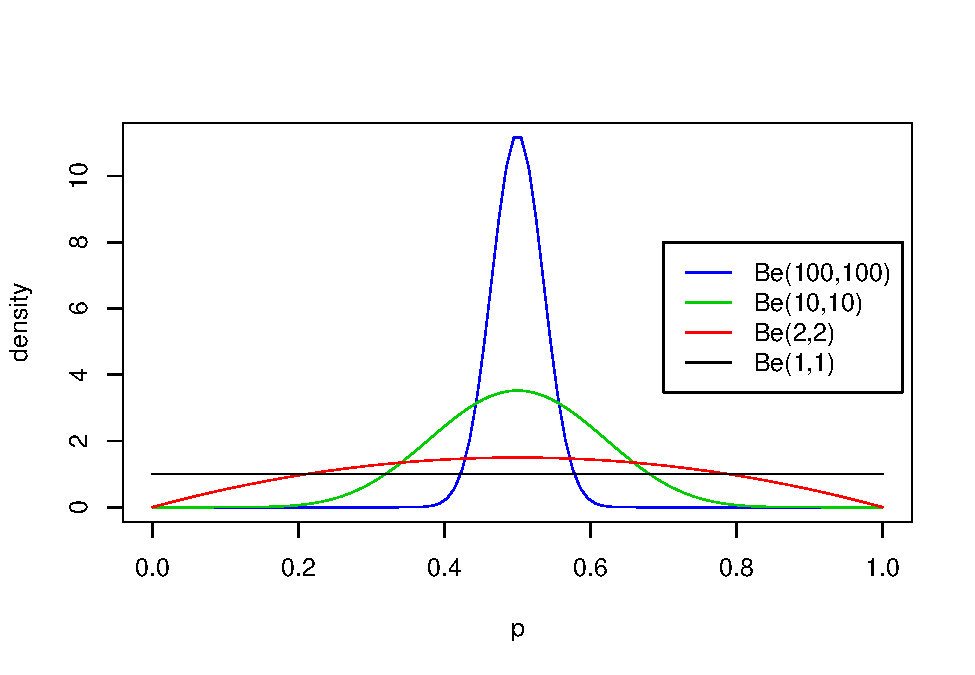
\includegraphics{ulupaper2009_files/figure-latex/unnamed-chunk-2-1.pdf}
\#\#\#\# non-equal alpha and beta:

\begin{Shaded}
\begin{Highlighting}[]
\NormalTok{p =}\StringTok{ }\KeywordTok{seq}\NormalTok{(}\DecValTok{0}\NormalTok{,}\DecValTok{1}\NormalTok{, }\DataTypeTok{length=}\DecValTok{100}\NormalTok{)}
\KeywordTok{plot}\NormalTok{(p, }\KeywordTok{dbeta}\NormalTok{(p, }\DecValTok{900}\NormalTok{, }\DecValTok{100}\NormalTok{), }\DataTypeTok{ylab=}\StringTok{"density"}\NormalTok{, }\DataTypeTok{type =}\StringTok{"l"}\NormalTok{, }\DataTypeTok{col=}\DecValTok{4}\NormalTok{)}
\KeywordTok{lines}\NormalTok{(p, }\KeywordTok{dbeta}\NormalTok{(p, }\DecValTok{90}\NormalTok{, }\DecValTok{10}\NormalTok{), }\DataTypeTok{type =}\StringTok{"l"}\NormalTok{, }\DataTypeTok{col=}\DecValTok{3}\NormalTok{)}
\KeywordTok{lines}\NormalTok{(p, }\KeywordTok{dbeta}\NormalTok{(p, }\DecValTok{30}\NormalTok{, }\DecValTok{70}\NormalTok{), }\DataTypeTok{col=}\DecValTok{2}\NormalTok{) }
\KeywordTok{lines}\NormalTok{(p, }\KeywordTok{dbeta}\NormalTok{(p, }\DecValTok{3}\NormalTok{, }\DecValTok{7}\NormalTok{), }\DataTypeTok{col=}\DecValTok{1}\NormalTok{) }
\KeywordTok{legend}\NormalTok{(}\FloatTok{0.2}\NormalTok{,}\DecValTok{30}\NormalTok{, }\KeywordTok{c}\NormalTok{(}\StringTok{"Be(900,100)"}\NormalTok{,}\StringTok{"Be(90,10)"}\NormalTok{,}\StringTok{"Be(30,70)"}\NormalTok{, }\StringTok{"Be(3,7)"}\NormalTok{),}\DataTypeTok{lty=}\KeywordTok{c}\NormalTok{(}\DecValTok{1}\NormalTok{,}\DecValTok{1}\NormalTok{,}\DecValTok{1}\NormalTok{,}\DecValTok{1}\NormalTok{),}\DataTypeTok{col=}\KeywordTok{c}\NormalTok{(}\DecValTok{4}\NormalTok{,}\DecValTok{3}\NormalTok{,}\DecValTok{2}\NormalTok{,}\DecValTok{1}\NormalTok{))}
\end{Highlighting}
\end{Shaded}

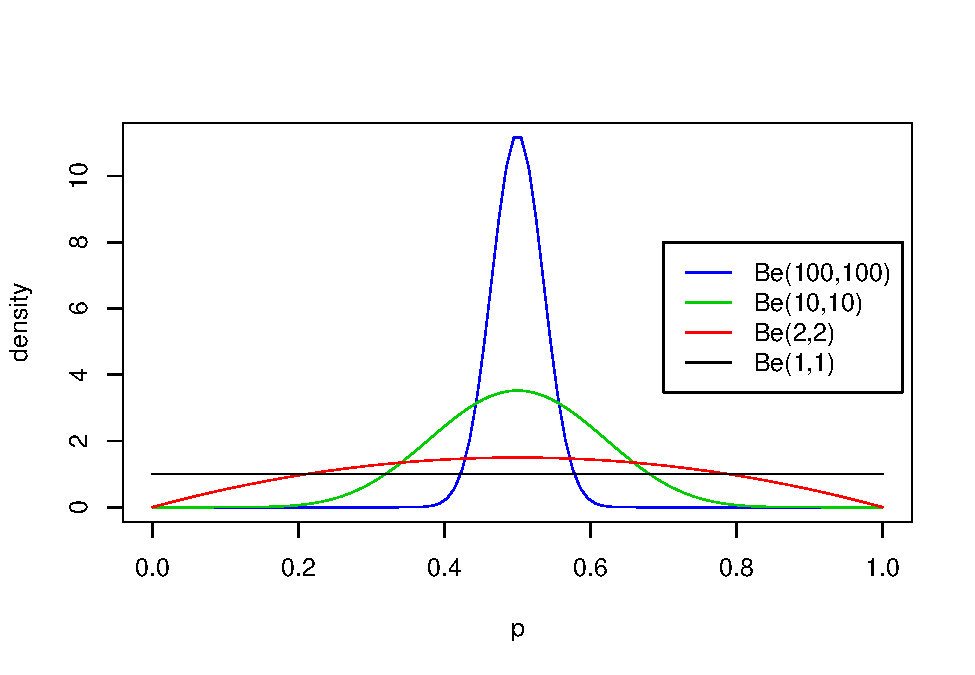
\includegraphics{ulupaper2009_files/figure-latex/unnamed-chunk-3-1.pdf}

Two points about the \emph{Beta} distribution:

From these examples you should note the following:
\[E[p]=\frac{\alpha}{\alpha+\beta}\]
* It turns out that the mean is exactly Thus the mean of the distribution is determined by the relative values of a and b.

\begin{itemize}
\tightlist
\item
  The larger the values of a and b, the smaller the variance of the distribution about the mean.
\end{itemize}

\[Var[p]=E[(X-\mu)^2]=\frac{\alpha\beta}{(\alpha+\beta)^2(\alpha+\beta+1)}\]

\hypertarget{alpha-and-beta-1}{%
\subsubsection{alpha and beta \textless1}\label{alpha-and-beta-1}}

\begin{Shaded}
\begin{Highlighting}[]
\NormalTok{p =}\StringTok{ }\KeywordTok{seq}\NormalTok{(}\DecValTok{0}\NormalTok{,}\DecValTok{1}\NormalTok{, }\DataTypeTok{length=}\DecValTok{100}\NormalTok{)}
\KeywordTok{plot}\NormalTok{(p, }\KeywordTok{dbeta}\NormalTok{(p, }\FloatTok{0.9}\NormalTok{, }\FloatTok{0.1}\NormalTok{), }\DataTypeTok{ylab=}\StringTok{"density"}\NormalTok{, }\DataTypeTok{type =}\StringTok{"l"}\NormalTok{, }\DataTypeTok{col=}\DecValTok{4}\NormalTok{)}
\KeywordTok{lines}\NormalTok{(p, }\KeywordTok{dbeta}\NormalTok{(p, }\FloatTok{0.7}\NormalTok{, }\FloatTok{0.3}\NormalTok{), }\DataTypeTok{type =}\StringTok{"l"}\NormalTok{, }\DataTypeTok{col=}\DecValTok{3}\NormalTok{)}
\KeywordTok{lines}\NormalTok{(p, }\KeywordTok{dbeta}\NormalTok{(p, }\FloatTok{0.5}\NormalTok{, }\FloatTok{0.7}\NormalTok{), }\DataTypeTok{col=}\DecValTok{2}\NormalTok{) }
\KeywordTok{lines}\NormalTok{(p, }\KeywordTok{dbeta}\NormalTok{(p, }\FloatTok{0.3}\NormalTok{, }\FloatTok{0.9}\NormalTok{), }\DataTypeTok{col=}\DecValTok{1}\NormalTok{) }
\KeywordTok{legend}\NormalTok{(}\FloatTok{0.2}\NormalTok{,}\DecValTok{4}\NormalTok{, }\KeywordTok{c}\NormalTok{(}\StringTok{"Be(0.9,0.1)"}\NormalTok{,}\StringTok{"Be(0.7,0.3)"}\NormalTok{,}\StringTok{"Be(0.5,0.7)"}\NormalTok{, }\StringTok{"Be(0.3,0.9)"}\NormalTok{), }\DataTypeTok{col=}\KeywordTok{c}\NormalTok{(}\DecValTok{4}\NormalTok{,}\DecValTok{3}\NormalTok{,}\DecValTok{2}\NormalTok{,}\DecValTok{1}\NormalTok{), }\DataTypeTok{lty=}\KeywordTok{c}\NormalTok{(}\DecValTok{1}\NormalTok{,}\DecValTok{1}\NormalTok{,}\DecValTok{1}\NormalTok{,}\DecValTok{1}\NormalTok{))}
\end{Highlighting}
\end{Shaded}

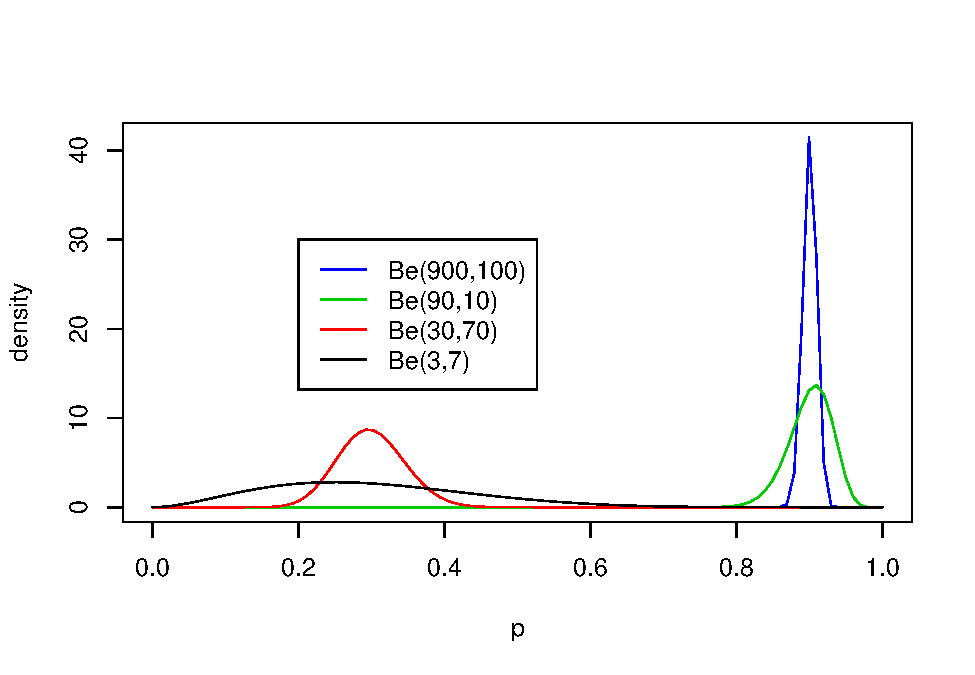
\includegraphics{ulupaper2009_files/figure-latex/unnamed-chunk-4-1.pdf}

\hypertarget{beta-conjugate-to-bernoulli-distibutaion}{%
\section{Beta Conjugate to Bernoulli Distibutaion}\label{beta-conjugate-to-bernoulli-distibutaion}}

\hypertarget{prior}{%
\subsection{Prior:}\label{prior}}

\[Beta(\alpha,\beta) = \frac{\theta^{\alpha-1}(1-\theta)^{\beta-1}}{B(\alpha,\beta)}\]

\[= const.\theta^{\alpha-1}(1-\theta)^{b-1}\]

\hypertarget{posterior-distribution}{%
\subsection{Posterior Distribution:}\label{posterior-distribution}}

\[P(\theta|data)=\frac{P(data|\theta)P(\theta)}{P(data)}\propto P(data|\theta)P(theta)\]

\hypertarget{beta-binomial-model}{%
\section{Beta-Binomial Model}\label{beta-binomial-model}}

\hypertarget{likelihood}{%
\subsection{Likelihood:}\label{likelihood}}

\[P(data|\theta) \propto \theta^z(1-\theta)^{n-z},\]
if we let z number of \(x_{i}\) with value 1, i.e, (seeing z success in n trial)

\[z=\sum_{i=1}^{n}X_i\]

\hypertarget{derive-posterior}{%
\subsection{Derive Posterior}\label{derive-posterior}}

\[P(\theta|data) \propto ( \theta^z(1-\theta)^{n-z})(\theta^{\alpha-1}(1-\theta)^{\beta-1})\]\\
\[\propto \theta^{z+\alpha-1}(1-\alpha)^{n-z+\beta-1}\]
Subsituing the following:

\[\alpha'=\alpha + z\]
\[\beta'=n+\beta-z\]
Now we have posterior:

\[P(\theta | data) = \frac{\theta^{\alpha'-1}(1-\alpha)^{\beta'-1}}{B(\alpha',\beta')}\]

\[=Beta(\alpha',\beta')\]

\hypertarget{example-of-the}{%
\section{Example of the:}\label{example-of-the}}

\hypertarget{prior-1}{%
\subsection{Prior}\label{prior-1}}

Beta with \(\alpha\)=1, \(\beta\)=1:

\begin{Shaded}
\begin{Highlighting}[]
\NormalTok{N \textless{}{-}}\StringTok{ }\DecValTok{1000}
\NormalTok{alpha \textless{}{-}}\StringTok{ }\DecValTok{1}
\NormalTok{beta \textless{}{-}}\StringTok{ }\DecValTok{1}
\NormalTok{nsuccess \textless{}{-}}\StringTok{ }\DecValTok{2}
\NormalTok{n\_trials \textless{}{-}}\StringTok{ }\DecValTok{4}

\NormalTok{data\_}\DecValTok{1}\NormalTok{\_}\DecValTok{1}\NormalTok{ \textless{}{-}}\StringTok{ }\KeywordTok{tibble}\NormalTok{(}\DataTypeTok{p\_grid =} \KeywordTok{seq}\NormalTok{(}\DataTypeTok{from=}\DecValTok{0}\NormalTok{, }\DataTypeTok{to =}\DecValTok{1}\NormalTok{, }\DataTypeTok{length.out =}\NormalTok{ N)) }\OperatorTok{\%\textgreater{}\%}\StringTok{ }
\StringTok{  }\KeywordTok{mutate}\NormalTok{(}\DataTypeTok{prior=}\KeywordTok{dbeta}\NormalTok{(p\_grid,alpha,beta)) }\OperatorTok{\%\textgreater{}\%}\StringTok{ }
\StringTok{  }\KeywordTok{mutate}\NormalTok{(}\DataTypeTok{likelihood =} \KeywordTok{dbinom}\NormalTok{(nsuccess, }\DataTypeTok{size =}\NormalTok{ n\_trials, }\DataTypeTok{prob =}\NormalTok{ p\_grid)) }\OperatorTok{\%\textgreater{}\%}\StringTok{ }
\StringTok{  }\KeywordTok{mutate}\NormalTok{(}\DataTypeTok{posterior =}\NormalTok{ (likelihood }\OperatorTok{*}\StringTok{ }\NormalTok{prior) }\OperatorTok{/}\StringTok{ }\KeywordTok{sum}\NormalTok{(likelihood }\OperatorTok{*}\StringTok{ }\NormalTok{prior))}
\end{Highlighting}
\end{Shaded}

\begin{Shaded}
\begin{Highlighting}[]
\NormalTok{data\_}\DecValTok{1}\NormalTok{\_}\DecValTok{1} \OperatorTok{\%\textgreater{}\%}\StringTok{ }
\StringTok{  }\KeywordTok{gather}\NormalTok{(key, value, }\OperatorTok{{-}}\NormalTok{p\_grid) }\OperatorTok{\%\textgreater{}\%}\StringTok{  }
\StringTok{  }\CommentTok{\# this line allows us to dictate the order the panels will appear in}
\StringTok{  }\KeywordTok{mutate}\NormalTok{(}\DataTypeTok{key =} \KeywordTok{factor}\NormalTok{(key, }\DataTypeTok{levels =} \KeywordTok{c}\NormalTok{(}\StringTok{"prior"}\NormalTok{, }\StringTok{"likelihood"}\NormalTok{, }\StringTok{"posterior"}\NormalTok{))) }\OperatorTok{\%\textgreater{}\%}\StringTok{ }
\StringTok{  }\KeywordTok{ggplot}\NormalTok{(}\KeywordTok{aes}\NormalTok{(}\DataTypeTok{x =}\NormalTok{ p\_grid, }\DataTypeTok{ymin =} \DecValTok{0}\NormalTok{, }\DataTypeTok{ymax =}\NormalTok{ value, }\DataTypeTok{fill =}\NormalTok{ key)) }\OperatorTok{+}
\StringTok{  }\KeywordTok{geom\_ribbon}\NormalTok{() }\OperatorTok{+}
\StringTok{  }\KeywordTok{scale\_fill\_manual}\NormalTok{(}\DataTypeTok{values =} \KeywordTok{c}\NormalTok{(}\StringTok{"blue"}\NormalTok{, }\StringTok{"red"}\NormalTok{, }\StringTok{"purple"}\NormalTok{)) }\OperatorTok{+}
\StringTok{  }\KeywordTok{scale\_y\_continuous}\NormalTok{(}\OtherTok{NULL}\NormalTok{, }\DataTypeTok{breaks =} \OtherTok{NULL}\NormalTok{) }\OperatorTok{+}
\StringTok{  }\KeywordTok{theme}\NormalTok{(}\DataTypeTok{legend.position =} \StringTok{"none"}\NormalTok{) }\OperatorTok{+}
\StringTok{  }\KeywordTok{facet\_wrap}\NormalTok{(}\OperatorTok{\textasciitilde{}}\NormalTok{key, }\DataTypeTok{scales =} \StringTok{"free"}\NormalTok{)}
\end{Highlighting}
\end{Shaded}

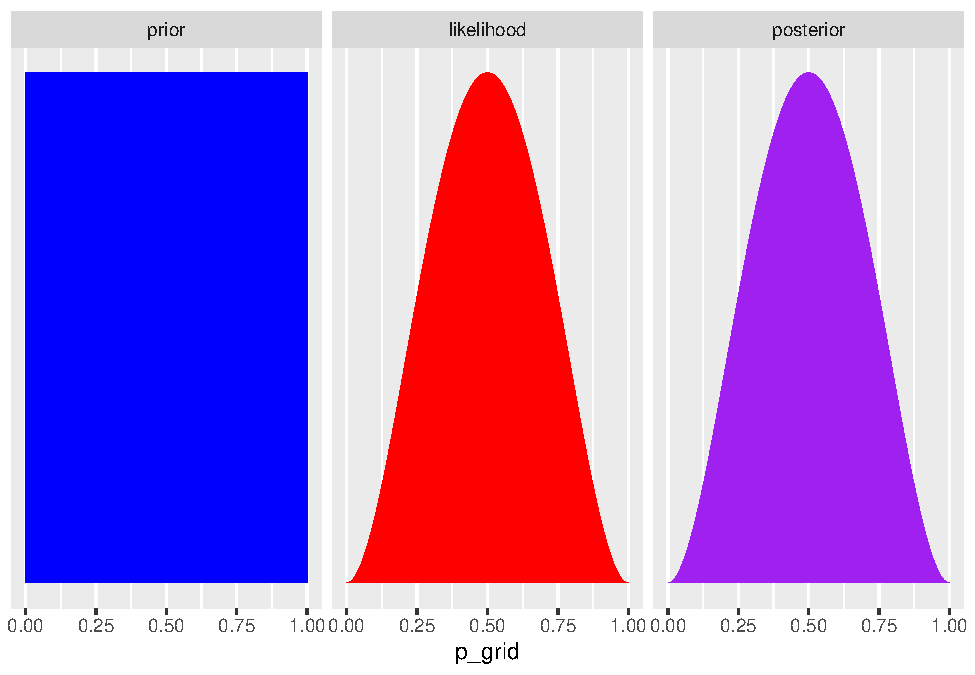
\includegraphics{ulupaper2009_files/figure-latex/unnamed-chunk-6-1.pdf}

Analytically, the mean of the posterior should be:

\[Beta(\alpha + s, \beta + n -s)\]
with mean value of

\[E[X]=\frac{\alpha + s}{\alpha + \beta + n}\]
having \(\alpha\)=1, \(\beta=1\), \(s\)=2 and \(n\)=4 :

\[Beta(1 + 2, 1+ 4-2)\]
\[Beta(3, 3)\]
with mean value of

\[E[pgrid]=\frac{3}{3+6}=\frac{1}{3}\]

\hypertarget{normal-normal-conjugate}{%
\section{Normal-Normal Conjugate:}\label{normal-normal-conjugate}}

\[P(\theta | Data) = \frac{P(Data|\theta)P(\theta)}{P(Data)} \propto P(Data|\theta)P(\theta)\]
\[P(Data|\theta) = \prod_{i=1}^{N}\frac{1}{\sqrt{2\pi\sigma_x^2}}exp(-\frac{(x_i-\theta)²}{2\sigma_x^2})\]
\[\propto exp(-\frac{\sum_{i=1}^{N}(x_i-\theta)^2}{2\sigma_x^2})\]
Now posterior:

\[P(\theta|X) \propto  exp(-\frac{\sum_{i=1}^{N}(x_i-\theta)^2}{2\sigma_x^2})exp(-\frac{(\theta-\theta_0)^2}{2\sigma_{\theta}^2})\]
\[=exp[-\]
You can label chapter and section titles using \texttt{\{\#label\}} after them, e.g., we can reference Chapter \ref{intro}. If you do not manually label them, there will be automatic labels anyway, e.g., Chapter \ref{methods}.

Figures and tables with captions will be placed in \texttt{figure} and \texttt{table} environments, respectively.

\begin{Shaded}
\begin{Highlighting}[]
\KeywordTok{par}\NormalTok{(}\DataTypeTok{mar =} \KeywordTok{c}\NormalTok{(}\DecValTok{4}\NormalTok{, }\DecValTok{4}\NormalTok{, }\FloatTok{.1}\NormalTok{, }\FloatTok{.1}\NormalTok{))}
\KeywordTok{plot}\NormalTok{(pressure, }\DataTypeTok{type =} \StringTok{\textquotesingle{}b\textquotesingle{}}\NormalTok{, }\DataTypeTok{pch =} \DecValTok{19}\NormalTok{)}
\end{Highlighting}
\end{Shaded}

\begin{figure}

{\centering 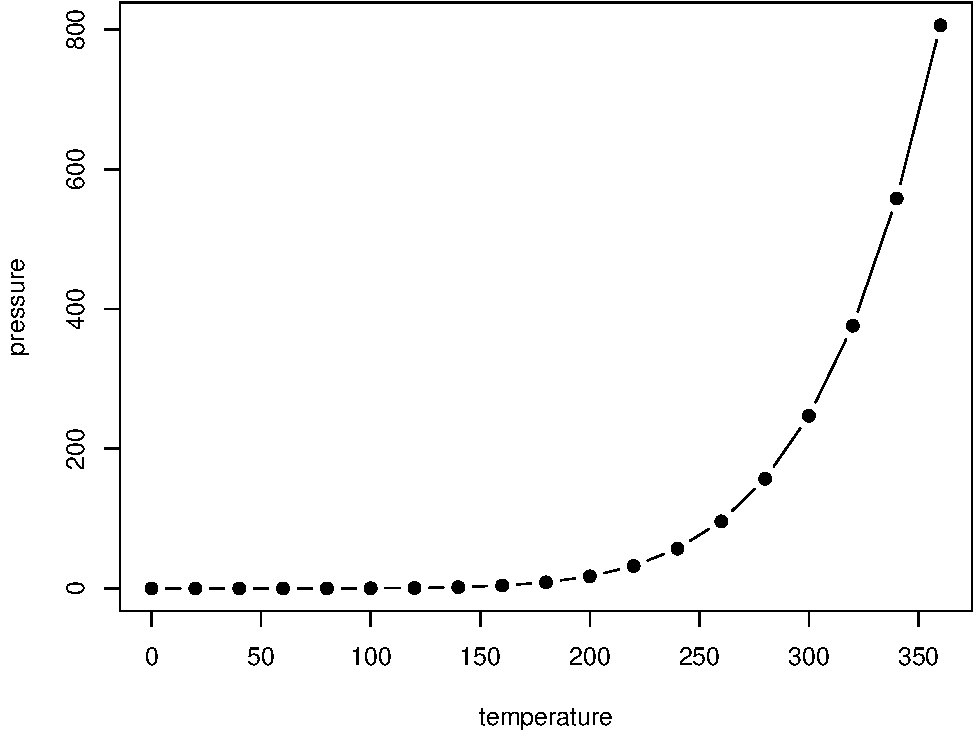
\includegraphics[width=0.8\linewidth]{ulupaper2009_files/figure-latex/nice-fig-1} 

}

\caption{Here is a nice figure!}\label{fig:nice-fig}
\end{figure}

Reference a figure by its code chunk label with the \texttt{fig:} prefix, e.g., see Figure \ref{fig:nice-fig}. Similarly, you can reference tables generated from \texttt{knitr::kable()}, e.g., see Table \ref{tab:nice-tab}.

\begin{Shaded}
\begin{Highlighting}[]
\NormalTok{knitr}\OperatorTok{::}\KeywordTok{kable}\NormalTok{(}
  \KeywordTok{head}\NormalTok{(iris, }\DecValTok{20}\NormalTok{), }\DataTypeTok{caption =} \StringTok{\textquotesingle{}Here is a nice table!\textquotesingle{}}\NormalTok{,}
  \DataTypeTok{booktabs =} \OtherTok{TRUE}
\NormalTok{)}
\end{Highlighting}
\end{Shaded}

\begin{table}

\caption{\label{tab:nice-tab}Here is a nice table!}
\centering
\begin{tabular}[t]{rrrrl}
\toprule
Sepal.Length & Sepal.Width & Petal.Length & Petal.Width & Species\\
\midrule
5.1 & 3.5 & 1.4 & 0.2 & setosa\\
4.9 & 3.0 & 1.4 & 0.2 & setosa\\
4.7 & 3.2 & 1.3 & 0.2 & setosa\\
4.6 & 3.1 & 1.5 & 0.2 & setosa\\
5.0 & 3.6 & 1.4 & 0.2 & setosa\\
\addlinespace
5.4 & 3.9 & 1.7 & 0.4 & setosa\\
4.6 & 3.4 & 1.4 & 0.3 & setosa\\
5.0 & 3.4 & 1.5 & 0.2 & setosa\\
4.4 & 2.9 & 1.4 & 0.2 & setosa\\
4.9 & 3.1 & 1.5 & 0.1 & setosa\\
\addlinespace
5.4 & 3.7 & 1.5 & 0.2 & setosa\\
4.8 & 3.4 & 1.6 & 0.2 & setosa\\
4.8 & 3.0 & 1.4 & 0.1 & setosa\\
4.3 & 3.0 & 1.1 & 0.1 & setosa\\
5.8 & 4.0 & 1.2 & 0.2 & setosa\\
\addlinespace
5.7 & 4.4 & 1.5 & 0.4 & setosa\\
5.4 & 3.9 & 1.3 & 0.4 & setosa\\
5.1 & 3.5 & 1.4 & 0.3 & setosa\\
5.7 & 3.8 & 1.7 & 0.3 & setosa\\
5.1 & 3.8 & 1.5 & 0.3 & setosa\\
\bottomrule
\end{tabular}
\end{table}

You can write citations, too. For example, we are using the \textbf{bookdown} package \citep{R-bookdown} in this sample book, which was built on top of R Markdown and \textbf{knitr} \citep{xie2015}. change new line

\hypertarget{literature}{%
\chapter{Literature}\label{literature}}

\hypertarget{to-do}{%
\section{To Do}\label{to-do}}

\hypertarget{methods}{%
\chapter{Methods}\label{methods}}

\hypertarget{to-do-1}{%
\section{To DO}\label{to-do-1}}

\hypertarget{applications}{%
\chapter{Applications}\label{applications}}

\hypertarget{to-do-2}{%
\section{To DO!}\label{to-do-2}}

\hypertarget{final-words}{%
\chapter{Final Words}\label{final-words}}

\hypertarget{to-do-3}{%
\section{To Do!}\label{to-do-3}}

  \bibliography{Phd-Literature.bib,packages.bib}

\end{document}
